\section{Tiền xử lý số liệu}
\subsection{Đọc dữ liệu}
Đầu tiên, ta tiến hành đọc tệp tin "dirty$\_$data.csv" vào RStudio với dữ liệu được lấy từ \href{https://www.kaggle.com/datasets/muhammadshahrayar/transactional-retail-dataset-of-electronics-store?select=dirty_data.csv}{Kaggle} và kiểm tra một số thông tin về tệp tin với câu lệnh chính được sử dụng là \textbf{text.csv}(\textbf{Code[1]$\rightarrow$[2]}).

\begin{figure}[H]
    \centering
    
\includegraphics[scale =0.5]{IMAGES/1.png}
    \caption{Kết quả khi kiểm tra một số thông tin về tệp tin}
    \label{fig1}
\end{figure}
\textbf{\textit{Nhận xét}}: Hình~\ref{fig1} Nhìn vào bảng ta thấy được dữ liệu được nạp vào tệp giống với các biến trong phần tổng quan về dữ liệu bao gồm 16 biến và 500 quan trắc.
\subsection{Làm sạch dữ liệu}
Ta tiến hành tạo tệp tin con bao gồm 11 biến bao gồm biên liên tục và biến phân loại cần phân tích để xem xét sự ảnh hưởng của biến order\_total với 11 biến trên và xem 10 dòng đầu. Những biến đó bao gồm order\_total, order\_price, delivery\_charges, coupon\_discount, season, is\_expedited\_delivery, is\_happy\_customer, distance\_to\_nearest\_warehouse, customer\_lat và customer\_long  (\textbf{Code[4]$\rightarrow$[6]}).
\begin{figure}[H]
    \centering
    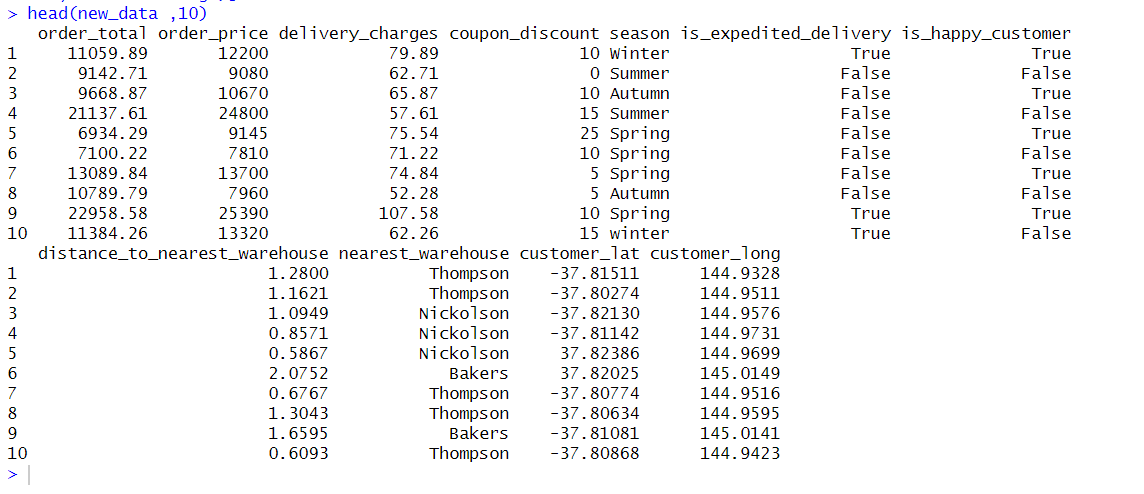
\includegraphics[scale =0.5]{IMAGES/34.png}
    \caption{Kết quả khi kiểm tra một số thông tin về tệp tin}
    \label{fig2}
\end{figure}

Sau đó, ta cần kiểm tra những dữ liệu bị khuyết với lệnh chính \textbf{head} để kết quả sau khi phân tích dữ liệu được chính xác hơn (\textbf{Code[7]$\rightarrow$[9]}).
\begin{figure}[H]
    \centering
    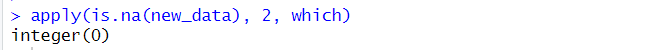
\includegraphics[width=0.7\linewidth]{IMAGES/35.png}
    \caption{Kết quả khi kiểm tra dữ liệu khuyết}
    \label{fig3}
\end{figure}
\textbf{\textit{Nhận xét}}: Hình~\ref{fig3} Sau khi kiểm tra, ta thấy được tệp không có dữ liệu khuyết. Sau đó, ta tiến hành kiểm tra biến season (\textbf{Code[10]}). 
\begin{figure}[H]
    \centering
    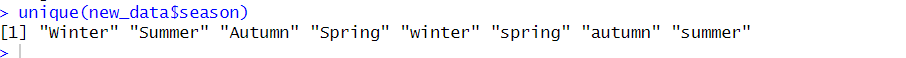
\includegraphics[width=0.8\linewidth]{IMAGES/36.png}
    \caption{Kết quả khi kiểm tra biến season}
    \label{fig04}
\end{figure}

\textbf{\textit{Nhận xét}}: Hình~\ref{fig04} Kết quả kiểm tra cho thấy biến có lỗi định dạng, ta thực hiện thay các giá trị "spring" = "Spring", "summer" = "Summer", "autum" = "Autum", "winter" = "Winter" bằng hàm gán  và kiểm tra kết quả (\textbf{Code[12]$\rightarrow$[16]}).  
\begin{figure}[H]
    \centering
    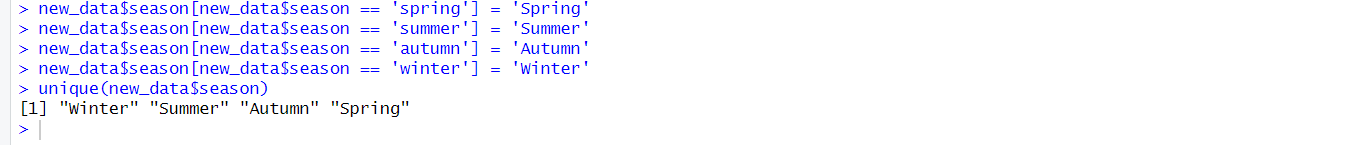
\includegraphics[width=0.9\linewidth]{
    IMAGES/a.png}
    \caption{Kết quả khi kiểm tra lại các giá trị của season.}
    \label{fig5}
\end{figure}
\textbf{\textit{Nhận xét}}: Hình~\ref{fig5} Như vậy, sau khi thay các giá trị của biến season ta thấy được biến season đã cho ra định dạng như ta mong muốn.
Ta tiếp tục nhận thấy biến season và date đang có sự sai lệch với nhau. Ngoài ra, ta nhận thấy được định dạng của ngày-tháng-năm đang không được đồng nhất. Ta điều chỉnh định dạng của ngày-tháng-năm thành \%Y-\%m-\%d  và điều chỉnh season theo đúng với ngày  bằng lệnh điều kiện (\textbf{ifelse}) và hàm gán. Ví dụ: tháng 6 là mùa hè (Summer) nhưng trong dữ liệu lại là mùa xuân (Spring) (\textbf{Code[18]$\rightarrow$[21]}). 
\begin{figure}[H]
    \centering
    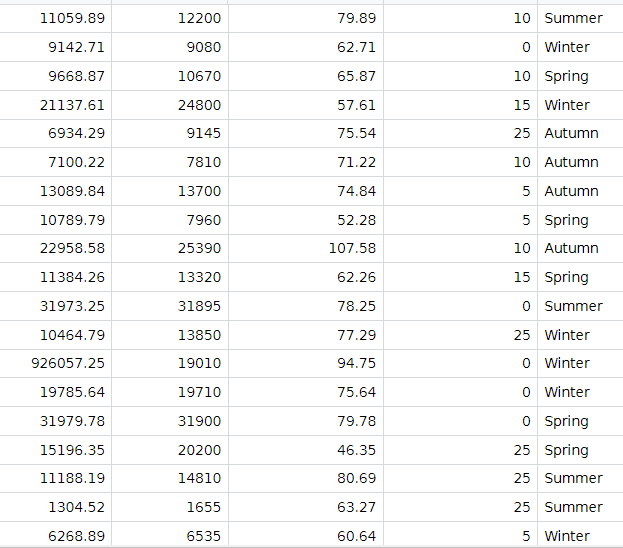
\includegraphics[scale=0.5]{
    IMAGES/37.png}
    \caption{Kết quả khi kiểm tra và điều chỉnh lại season theo date.}
    \label{fig6}
\end{figure}
\textbf{\textit{Nhận xét}}: Hình~\ref{fig6}: Như vậy, kết quả của giá trị season theo biến date cho ra đã đúng định dạng mà ta mong muốn.
Tiếp tục, ta kiểm tra biến nearest\_warehouse (\textbf{Code[23]}). 
\begin{figure}[H]
    \centering
    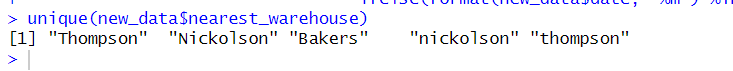
\includegraphics[width=0.8\linewidth]{
    IMAGES/38.png}
    \caption{Kết quả khi kiểm tra biến nearest\_warehouse.}
    \label{fig7}
\end{figure}
\textbf{\textit{Nhận xét}}: Hình~\ref{fig7} Ta thấy được biến nearest\_warehouse đang có nhiều định dạng khác nhau dẫn đến sai lệch khi phân tích. Ta tiến hành điều chỉnh lại định dạng nickolson=Nickolson, thompson=Thompson bằng hàm gán. (\textbf{Code[24]$\rightarrow$[26]}).
\begin{figure}[H]
    \centering
    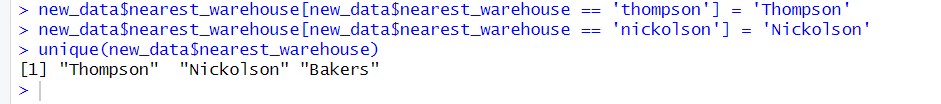
\includegraphics[width=0.8\linewidth]{
    IMAGES/39.png}
    \caption{Kết quả sau khi điều chỉnh biến nearest\_warehouse.}
    \label{fig8}
\end{figure}
\textbf{\textit{Nhận xét}}: Hình~\ref{fig8} Như vậy, biến nearest\_warehouse đã cho ra 4 định dạng như ta mong muốn.


Như vậy, dữ liệu đã được làm sạch hoàn toàn, ta tiến hành phân tích.